\documentclass[border=3mm]{standalone}
\usepackage{tikz}
\usetikzlibrary{calc,circuits.ee.IEC}

\begin{document}
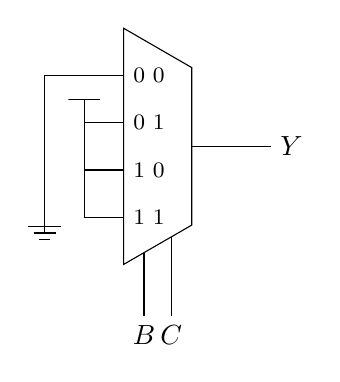
\begin{tikzpicture}[circuit ee IEC,small circuit symbols]

% Mux body.
\draw (0,0)coordinate (O)--++(30:1)coordinate (A)--++(90:2)coordinate (B)--++(150:1)coordinate (C)--cycle;

% Mux output.
\draw ($(A)!0.5!(B)$)--++(0:1)node[right]{$Y$};

% Mux input select.
\draw ($(O)!0.70!(A)$)--++(270:10mm)node[below]{$C$};
\draw ($(O)!0.30!(A)$)--++(270:8.0mm)node[below]{$B$};

% Loop for each mux terminal.
\foreach \y/\t/\b/\c in {0.1/0/0/0,0.2/1/0/1,0.3/2/1/0,0.4/3/1/1} {

    % Draw each terminal.
    \draw
        ($(C)! \y*2.0 !(O)$) -- ++(180:0.5cm)
        node(term\t)[anchor=center] {};

    % Draw binary numbers to select. End loop.
    \draw
        ($(C)! \y*2.0 !(O)$) ++ (0:0.0)
        node[right,font=\footnotesize] {$\b$ $\c$};
}

% Connect term3-term1 to Vdd
\draw
    % start center of last term node
    (term3.center)
    % draw line to node term1 center
    -- (term1.center)
    % extend and make vdd symbol with
    % back and forth squiggle
    -- ++(90:3mm) -- ++(180:2mm) -- ++(0:4mm);

\draw (term0.center) -- ++(180:-0.0cm) -- ++(180:0.5cm) -- ++(270:2)node[ground={pos=1},point down]{};
\end{tikzpicture}
\end{document}
